% TITLE PAGE
% ABSTRACT

% 10-20 PAGES INCLUDING:
	% Contextual Information - Lit Review
	% Process Information - Goals and Methods
	% Reflections - Learned, Retrospective, Implications

\documentclass[titlepage]{article}
\usepackage{graphicx} % Required for inserting images
\usepackage{setspace} % Used to set double spacing
\usepackage[margin=1in]{geometry} % Sets margins to 1 inch
\usepackage{ textcomp } % Angle brackets
\usepackage{tikz} % For diagrams
\usepackage{wrapfig} % For wrapping around figures

% CODE BLOCK DEFINITIONS
\usepackage{listings}
\usepackage{courier}
\lstset{
	breaklines=true,
	columns=fixed,
	basicstyle=\ttfamily,
	basewidth=0.5em,
	frame=tlrb
}
\lstnewenvironment{codeblock}[1][]
	{\lstset{#1}\noindent\minipage{6.5in}}
	{\endminipage}

\newcommand{\lstRef}[1]{Listing \ref{lst:#1}}

% LANGUAGE NAME
\newcommand{\langName}{Vizzini}

% SET DOUBLE SPACING
\doublespacing{}

% TITLE DEFINITION
\title{Say ``Hello World!''.}
\author{Sandro Ansari}
\date{May 2025}

\begin{document}
% TITLE PAGE
\maketitle

% ABSTRACT
\begin{abstract}
	\langName{} is a programming language that looks like natural language. Leveraging React with Vue and Microsoft's ts-parsec library, the goal of this project was to show that a programming language can be made to look like English. Not only that, but on a fundamental level, the interpreter for \langName{} relies on semantic composition in order to derive the meaning of its sentences. While this type of language is largely inefficient, there are benefits in accessibility and interesting tie-ins with the field of semantics.
\end{abstract}

% MAIN BODY
\section*{Background}
The simplest way to describe my project is a programming language which appears naturalistic. The original programming languages were punch-card based and tied in to the machinery they worked on. Since then, new languages have evolved from low level machine code into higher level abstracted systems. The evolution from Fortran to C to Python (to name a few) showcases how languages have moved in a direction allowing for programmers to more abstractly tell the computer what to do. \langName{}\footnote{Named for the character in \textit{The Princess Bride} because of the language's verbosity and because sometimes things "[do not mean] what you think [they mean]"\cite{Goldman_1987}} is the natural next step in that evolution.

The original vision behind my project was being able to give the computer something that looked like pseudo-code and the machine would do the rest. Obviously, that is a herculean task. Semanticists do not even have an idea what a “chair” is. How on earth would I be able to teach a computer that. Programming languages also need to be deterministic for them to be useful, so leveraging large language models was out of the question. Thus I decided to steer away from these real language complexities while maintaining the benefits of readable, accessible code.

Instead of a natural language programming language, \langName{} was going to be a programming language wolf in natural language sheep's clothing. The grammar and lexicon would not match the scale of English by any means, but would offer a decent amount of variability in terms of grammatical framing. Programmers would be able to outline their programs in the way they like while keeping the program execution deterministic.

While a fully implemented natural programming language has the potential to solve many problems, the development of \langName{} pimarily focused on the problem of accessibility. Software developers are the first thought when it comes to programming, but many others need to use computers to accomplish complicated tasks in research and other areas. Many researchers use various programs to collect and analyze data, run simulations, and perform other tasks. However, for many, programming is not familiar or easy to grasp. In my own experience teaching programming to children at a summer camp, things as elementary as variables can be incredibly baffling when you've never been exposed to them.

A programming language that looks like a language you already speak can make working in that language easier for many reasons. You do not need to learn new syntax or keywords or modules or libraries. You can also understand others' code a lot easier if you can just read it like natural English.

This project has provided me an opportunity to explore syntax and semantics on the linguistics side of things while comparing those structures to analogous ones in programming syntax and structures. Figuring out how to allow for different frames of verbs or the multiple ways we talk about loops is the core intriguing component of this problem for me.

I have delved deep into parsers and semantic theory and learned how to make them work together. Having taken classes in syntax, semantics, and compilers, this is not an entirely new area for me, but my understanding of these topics has expanded beyond the scope of those classes. This has allowed me to assemble an artificial recreation of natural language with a lot of expressive power and flexibility.

Naturalistic programming languages have been attempted before with varying degrees of success and depth. My contribution to this field lies not in new goals but in the different strategies employed in my execution. Most projects I have found in this vein attempt to mimic and/or understand natural language in its entirety. This allows for a broader use of other natural languages or more idiomatic speech. \langName{} differs from these since it is first a programming language, the appearance of natural language being secondary. The main benefit of being accessible is preserved while the pitfalls of ambiguity and the incredible scope of natural language are avoided. \langName{} does not understand what you say but is rather a machine that does what it is told to do.

This approach does not offer as much expressive freedom as a fully implemented natural programming language but is still a useful tool. When you progress away from the machine level you lose efficiency. This project does not lose as much efficiency as a comprehensive naturalistic language since it is still a programming language (albeit with some very English-looking syntax). However, that is not to say it rivals C, but merely falls a bit closer to C than a language that suffers from the translation of English or some other language into code.

Being able to read, write, and share code efficiently and easily without much extra knowledge of syntax etc. makes for very effective and portable applications. As stated earlier, I am by no means the first to attempt this, so here is a sample of some previous efforts.

Many tools have looked to leverage natural language to various purposes. The language COBOL attempted to simulate English with its syntax \cite{Liu2005MetaforVS}. This meant defining control structures in a way that matched English framing as shown in \lstRef{cobolLoop}.

\begin{codeblock}[language=Cobol,caption={Cobol Loop Frame},label={lst:cobolLoop}]
PERFORM [n] TIMES
	[Statements]
END-PERFORM
\end{codeblock}

\lstRef{cobolLoop} somewhat mimics the English structure for talking about repeated actions. Other languages, including Python, also have syntax that can be somewhat read like English. Readability is important for people to quickly and easily understand code. However, some programming languages gone the extra mile.

Metafor is a project designed for outlining programming projects without over-committing to any given implementation \cite{Liu2005MetaforVS}. This project takes in natural language “stories” and creates outlines of classes and methods. It figures out which components ought to be properties and which ought to be classes among other things. This allows individuals to brainstorm without tying themselves to any particular structure. This means programmers can fail faster, and quickly prototype ideas.

Another approach was Pegasus \cite{Knöll2006PegasusFS}. Pegasus uses many advanced components including short-term memory to store context, long-term memory to store semantic information, and a way of matching all the components of the supplied sentence to those memories. It is a very sophisticated system that gets closer than many to the natural language ideal at the cost of some performance issues.

Pegasus and Metafor are closer to natural language than other programming languages in terms of their understanding of the input text. However other attempts simply try to mimic the appearance of natural language without the computer truly understanding the underlying linguistic phenomena the way Pegasus or Metaphor might, and these are only a few of the natural language programming languages that have been created (multiple of which are listed in Knöll \& Mezini).

Some of these experiments had interesting ideas applicable to my project. For example, a handful of them allow for fluffy constructions like “I would like …” or “Please …” These increase language flexibility and fluidity. Also, the ability to store the inflections of various words and assign specific meanings to them is very interesting. Not all of these features were feasible to add, but some more fundamental pieces like alternate grammatical frames and a semblance of real semantic composition make \langName{} more like English than many standard programming languages.

\section*{Goals}
The goals of \langName{} could be grouped into a few key groups: computational expressivity, natural language freedom, and linguistic fidelity. Balancing these three factors became a constant tug of war. Compromises had to be made in many places, but this push and pull of these three domains kept \langName{} focused on its true objective---becoming a programming language that looks like a natural language.

\subsection*{Computational Expressivity}
The first and most important aspect of a programming language is its ability to give instructions to a machine. An important metric here is whether or not the language is Turing complete. The Church-Turing thesis states that any problem solvable by an algorithm can be solved by a Turing machine (a model of computational device with exceptionally simple parameters). If a programming language can be used to simulate a Turing machine's actions, then it is proven that that language can solve any algorithmic problem.

In terms of expressive power, \langName{} being Turing complete is as good as any language can get. To prove that a language can simulate a Turing machine, instead of actually programming one, you can look at its features checking for branching control flow (if statements), looping control flow (while loops), and memory storage (variables). If all these features are present, then the language is Turing complete.

\subsection*{Natural Language Freedom}
This goal is the crux of the project. Users should have as much freedom with their input language as possible. The theoretical maximum of natural language freedom would be a language that can accept any valid sentences of English and work. Due to the scope of natural language, this is entirely unfeasible. However, there are a few features that have been included to support this goal. The most important one is alternative argument frames. In \langName{}, verbs take arguments just like in English. In English though, there are many ways of supplying those arguments to the verb. Allowing for multiple of these forms is the key way that \langName{} supports natural language freedom.

\subsection*{Linguistic Fidelity}
The last major goal was to incorporate as much real linguistic theory as possible to allow for increased language freedom and to offer a strong base for the parsing strategies \langName{} employs. This goal is critical when working with the first two. To allow for language freedom, I could have implemented a large number of manually created frames for all sorts of operations, but this would not be scalable and would make the computational expressivity limited to whatever those frames did. My actual approach leverages the lambda-calculus nature of natural language semantics to allow for exceptionally expressive sentences that are very English-like.

\section*{Planning}
Creating \langName{} has been a long and storied process with many ups and downs. The first step, as with many projects, is researching what others have done in the field. As mentioned earlier, the history of natural-looking languages is an eventful one. Starting with the advent of programming languages, programmers quickly began to bridge the computer-human communication gap. NLC is an unimplemented language designed by Bruce Ballard and Alan Biermann \cite{Ballard1979ProgrammingIN}. Their paper outlines a compelling argument for components a natural looking programming language needs and the types of data that such a language should be able to handle. Their model included a scanner, a parser, a semantic engine, and a matrix computer. \langName{} has the first three of these pieces as well. I utilize the ts-parsec library's built-in lexer and parser tools to tokenize the incoming sentences and then generate a pseudo-syntax tree. I can then run the top node of the tree and it will compose the meanings from across the syntax trees.

While NLC was a concept, as mentioned earlier, some other languages have gone above and beyond to reach true natural langauge parity. Pegasus stores concepts and ideas in a large network of terms and uses a complicated analysis of sentences at various levels to generate and execute the meaning of the input \cite{Knöll2006PegasusFS}. This system takes an incredibly comprehensive approach to natural langauge to the point where the program legitimately does its best to actually `understand' the input and resolve it according to its memory and background knowledge. The fact that a program can actually understand (as far as anything without consciousness can) what its being told to do is truly incredible.

Pegasus actually interpreting its input is in stark contrast with another popular avenue in this field AI. Artificial intelligences, large language models (LLMs) in particular, have grown incredibly strong in recent years in terms of their ability to understand natural language prompts. There are many tools now from GitHub Copilot to Claude AI that leverage these models and large amounts of online data to generate code for you based on simple pseudo-code-esque prompts. I knew from the beginning however, that this was not the direction I wanted to go. A programming language by definition, should make the computer do what its told to do. You should be able to clearly delineate the steps you want the machine to take. This should be true relative to the level of abstraction inherent to your language. In C++, you have to worry about pointers and memory allocation, and whatever you tell it to do, it will do (even if it inevitably causes a seg. fault). In Python, you do not need to worry about memory management, but if you tell it to print something it will do exactly that.

I did not want to use LLMs because they do not generate code that performs specific actions. Rather, these models will grab bits and pieces from all over the web to cobble together something that will only probably do what you want, and even if it does work, there's no guarantee it will do it in an efficient, or secure manner \cite{Fu2023SecurityWO}. This is a big factor in my goal of computational expressivity. Any user should be able to both write what they want the machine to do and have it completed accurately, and another should be able to read that person's code and know what it will do. This drove me in the direction of natural language parsers.

Initially I looked into the Spacy library for Python, the NLTK library (for various languages) and the Stanford Dependency Parser \cite{Marneffe2006GeneratingTD}. These parsers unfortunately did not mesh with my use-case for two reasons. First, the dependency parsers only did so much to give me a syntax tree. Dependencies do not directly translate to a semantically composable tree. Second, these parsers allowed for entirely too much freedom and thus would make it difficult to restrict the scope of allowable natural language. This was one situation in which natural language freedom was somewhat sacrificed for computational expressivity.

The last big step before beginning on the final version of \langName{} was some experiments with the context free grammar (CFG) parser from the NLTK library. I was successfully able to print strings and numbers as well as add and multiply numbers together.

\begin{codeblock}[caption={Initial CFG Sample},label={lst:CFGsample}]
> Say two times two.
: 4
> Say three plus four times thirty-five.
: 143
\end{codeblock}

This test gave me some useful insights into parsing with this CFG tool, but ultimately had a terrible flaw. I could not use any sort of state in the parsing. Variables and functions alike both rely on prior definitions that are accessible. If a parser cannot rely on these definitions, it makes it very difficult to guide the parser towards what a given verb needs. This led me to parser combinators.

Parser combinators are a strategy for building a parser out of small functions \cite{Hutton1996MonadicPC}. You are able to consume input and modify that consumed input to produce a tailored output. This is all expanded using a variety of higher order functions that combine these smaller pieces into exactly what you are looking for. This was the tool that allowed me to effectively create \langName{}.

The last decision I had to make before creating the final implementation was which language to write in. I had started this project with Python to roughly throw some ideas at the wall. Getting deeper into the weeds led me to consider a statically typed language moving forwards. This would help me to write more understandable code and generate less technical debt. For these reasons I decided to use TypeScript. This came with the added benefit of being able to use the React framework to create a streamlined and useful user interface. 

\section*{Product}
\subsection*{The Lexer}
The first layer of the \langName{} architecture is the lexer. This is a tool built using the ts-parsec library that groups the characters in the input into useful chunks. For my language, this meant words, numbers, and punctuation. Once I had these pieces I could further process them using the parser layer.

\subsection*{The Parser}
The parser layer is the largest and arguably most important component of \langName{}. The parser is split into three rough levels: literals and words, argument frames, and sentences. Together these three levels generate a tree of nodes that I call `XBars.' When the parser has parsed the full output with no errors, running the top XBar will perform the programmed instructions.

The literals and words level of the parser does two things. First, it resolves any words. This means taking the symbol (the character representation from the source) and looks it up in the current local lexicon. The parser also resolves number literals. In the original Python implementation, you could specify numbers using the word equivalent as in \lstRef{CFGsample}, but after moving to TypeScript, that feature has not been reimplemented. \langName{} does however work with both whole numbers and decimal numbers. The only other kind of literal currently parsable is strings. Strings can be delimited using matching single or double quotes. Strings also allow for escapable characters using the backslash.

\begin{codeblock}[caption={Lexer and Literal Parsing},label={lst:literalExample}]
> Say 2.
: {Say}{ }{2}{.}
> Bark.
: {Bark}{.}
> Say "Hello World!".
: {Say}{ }{"Hello World!"}{.}
> Say "My name is \"Sandro\"".
: {Say}{ }{"My name is \"Sandro\""}{.}
\end{codeblock}

The argument frame level is probably one of the most fundamentally important pieces of this entire project. This is the linchpin that allows for the natural language freedom that this language is trying to achieve. \langName{} reads sentences by first capturing a verb symbol, and then repeatedly accepting arguments. In order to account for the basic verbs that I have included in the default lexicon for \langName{}, I thought of a number of ways in which the arguments can be supplied to the verb using the rest of the sentence. The big example of flexibility comes in the form of variables. A key metric I used when judging a good framing was whether or not it sounded like English. Originally I just used variable names like variable names in other languages. However, telling somebody to "Say stuff" in English would have a person either say the word "stuff" or they might just say random words. It felt unintuitive for any old word to be usable as a variable name when English words already have their own meanings. Thus the ways to access variable values in \langName{} are ``the value of \textlangle\textit{varName}\textrangle" and ``\textlangle\textit{varName}\textrangle's value." My new guiding principle was not just whether it sounded like English but whether somebody new to programming would inherently understand what was happening. Telling somebody to "Save 2 as bob's value" makes a lot more sense than "Save 2 as bob."

The last level of the parser was the sentence and paragraph level. In \langName{}, sentences are split apart by punctuation like how other languages use semi-colons or linebreaks to delimit their lines. This means you can write a whole \langName{} program in one line if you wanted to. Sentences individually would grab a verb, all of the arguments it can and then a punctuation. The punctuation is actually composed with the rest of the meaning of the sentence. Periods don't change anything about the meaning, but colons supply the next sentence as an argument to the previous one.

\subsection*{The XBar Structure}
Now let us take a moment to explain how the XBars work in \langName{}. Every XBar node has a few key properties. First, it has a value. This value could be something like a string, a number, or boolean, or it could be something more complicated like a closure, or some more complicated function. That's where the second important piece of an XBar comes in. The type of an XBar's value is stored using a custom Semantic Type object. These come in three varieties: the simple type (string, void, number, etc.), the variable type (contains a dictionary of string:Semantic Type pairs), and the compound type (takes in a type and returns a type). By composing these types together, any type of an XBar can be described. The types can also be used to figure out whether nodes are able to compose with their sister nodes. Some types are also fuzzy which means they can match with multiple other types. The last important piece of data in an XBar is its children nodes. For a non-terminal node, semantic composition is used to generate its value based on these child nodes.

The XBar system I have employed is the primary way through which I adhere to the linguistic fidelity goal. By using semantic composition to derive the meaning of a sentence, these lines of code are actually working a lot more similarly to natural langauge than something like Python. Regular programming languages use CFG parsers to generate their code, but this is done through specific uses of parentheses, dots, and brackets. My strategy allows you to use any frames you want so long as they yield the correct types to compose.

This system relies heavily on the lexicon however and so far, my explanation has been hiding some under-the-hood tricks.

\subsection*{The Lexicon}
The lexicon is where the meanings of the sentence come from. The root of every sentence in \langName{} is the verb. This verbs definition comes from the lexicon tied to the scope the sentence is found within. Because the scope can change, everytime we reference a variable or verb, we need to make sure that the correct lexicon is being checked. Also, when a word is referenced, only the latest definition should be used. This meant that instead of creating an XBar with a number or string value whenever a variable name is referenced, instead we create an XBar that takes in a lexicon and returns a value. This was especially important considering loops. If you incremented  a value multiple times via a loop, you would only interpret the addition command once. If that does an operation based only on the initial state, than every operation will change the value to be exactly the same and nothing will be looped. If you resupply the current lexicon to the function each time, then the correct values are used.

\begin{codeblock}[caption={Scope Demonstration},label={lst:scopeDemo}]
> for each character in "abbc": if character's value is "b": for each letter in "def": Say character's value.
: b
: b
: b
: b
: b
: b
\end{codeblock}

\begin{wrapfigure}[7]{r}{2.1in}
	\hspace{1em}
	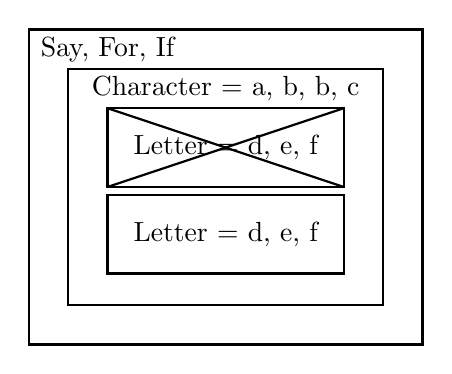
\begin{tikzpicture}
		\draw[black, thick] (0,-1) rectangle (5,3);
		\node at (1,2.75) {Say, For, If};
		\draw[black, thick] (.5,-.5) rectangle (4.5,2.5);
		\node at (2.5,2.25) {Character = a, b, b, c};
	
		\draw[black, thick] (1,1) rectangle (4,2);
		\node at (2.5,1.5) {Letter = d, e, f};
		\draw[black,thick] (1,1) to (4,2);
		\draw[black,thick] (4,1) to (1,2);
	
		\draw[black, thick] (1,-.1) rectangle (4,.9);
		\node at (2.5,0.4) {Letter = d, e, f};
	\end{tikzpicture}
\end{wrapfigure}

The shell's lexicon contains the verb definitions. A child lexicon is created within the shell lexicon for the outer for loop with a local variable stored as ``character's value.'' Then in the scenario where that value is ``e,'' the inner for loop creates an even deeper nested child lexicon within the current parent. For the second iteration of the outer loop, character's value will be set to ``b,'' and the inner loop will create a child lexicon. It does not reuse the old one. This diagram reflects the current state during the third iteration of the outer loop.

At any given point, you have access to the current lexicon. Some functions like ``For'' will send you into a child lexicon and then have you discard it afterwards. When referencing a verb or variable, the code will find the lowest version of that symbol in the current scope hierarchy. In this example, ``Say'' is only found at the top level, but when ``character'' is referenced, it only needs to go up one level.

\subsection*{Features}
\langName{} has a large number of features. These include:
\begin{itemize}
	\item Variable storing. Variables can be stored as ``the value of'' some name. In the future, it would be easy to extend this to objects by allowing more properties than just a ``value''. These variables can be stored and accessed using two different frames. First is the ``the value of [NAME]'' form and the second is the ``[NAME]'s value'' form.
	\item Printing. You can print values in \langName{} by telling it to ``Say'' something.
	\item If statements. There are actually two ways to use an if statement. The first is your classic if statement with an ``If'', a condition, and a colon followed by the if statement body. You can also do a terminal if statement, placing ``if'' and a condition at the end of your sentence.
	\item For loops. Like if statements, there is a classic for loop and a terminal for loop. Currently classic for loops are only used to iterate through a string. You start with ``For each'', then a name for the local iterator variable, then ``in'', and then the string you are iterating through followed by a colon and the loop body. The terminal for loop allows you to put ``[N] times'' at the end of your sentence in order to just run a simple sentence multiple times. `N' in this case could be a number or a variable with a number value.
	\item While loops. While loops have only a classic variant currently and follow the form ``While'', a condition, a colon, and then the loop body.
	\item Blocks. To create a connected block of code (e.g. to be used in a loop or if statement body), you only need to join the sentences together with ``, and'' instead of periods.
	\item Adding. The main operation that has been implemented in \langName{} is addition. You can add a number to a variable. Because negative numbers are valid, this means that subtraction is also implemented implicitly.
\end{itemize}

\section*{Discussion}
\langName{} is a complicated network of different systems that leverage computer science and linguistic principles and it fulfills my three core goals. First, with the inclusion of while loops, if statements, and variables, \langName{} is Turing complete. Meaning it satisfies the computational expressivity requirement. The deeply involved parser structure allows for the natural language freedom and helps facilitate the XBar system which in turn maintains linguistic fidelity. So, all the goals are accomplished. What makes this project useful?

There are many reasons why \langName{} is an important experiment in this field. First, it is the only project I've found so far that uses any notion of semantic composition. Second, This project sits in a sort of gap left between regular programming languages and languages more similar to Pegasus. By leveraging linguistic systems like semantic composition, \langName{} is able to look like Pegasus but work like Python. That combination is largely novel (at least with this implementation).

While this project is a large step in terms of natural-looking programming languages, it still falls victim to many of the usual challenges associated with programming languages and especially natural-looking ones. The farther away we get from the machine, the less efficient we can be when telling it what to do. Not only does this languages have inefficiencies due to many levels of abstraction, but it also suffers from inefficiencies directly related to the semantic model being employed. Composing each sentence and feeding it in a lexicon to generate the value is a slow process on the scale of computing. There are likely things that could be done to save time here and there, but the goal of this project was not peak efficiency. Even the changes that could be made would still leave performance lacking compared to regular programming languages.

It is also critical to note that this language has lots of room to expand. So many verbs and argument frames could be added to this language. What's more, it would not be entirely difficult. Each verb only requires you to creat its fundamental XBar (i.e. a value and a type). The level of specificity could also get more granular in future iterations. My parser tends to chunk certain words together (e.g. ``each \textlangle\textit{iterator}\textrangle\ in,'' ``the value of \textlangle\textit{variable}\textrangle''), but taken to extremes, you could imagine a lexicon where ``each,'' ``in,'' ``the,'' and ``of'' all have individual meanings. The other thing to note related to this is the fact that my parser for the most part only does branching in a certain direction. The verb is attached to the thing to its right, and then the next thing to the right is attached to that and so on. This means that complex argument structures don't really work. If you were to change how the parser worked to take into account other rules (e.g. phrase structure rules) or use a parsing algorithm accounting for composability with backtracking, you could get a lot closer to English with the programming language.

Another interesting implication of this project is the possibility of teaching applications. Having worked with young children learning to program, there are many things that a long-time programmer might take for granted. Variables being labels to store information under is not intuitive to somebody who has never seen something like that before. This is true for other structures in programming as well. If there were a language that let you talk to it in a way that explained what you were doing, that would likely help to reinforce how these different pieces work.

I do not think that \langName{} is the language of the future, but there are definitely a lot of features and ideas built into it that can be expanded upon and used in other systems. A language for learning that explains what it is doing without comments. A language for researchers that has lower barriers to entry. There are many possibilities, and they do not rely on incredibly complicated models of the brain or neural networks. That is the promise of \langName{}.


\newpage{}
\bibliographystyle{apalike}
\bibliography{Sources}

\end{document}